\documentclass{homework}
\usepackage{xcolor}
\usepackage{nicematrix}
\usepackage{booktabs}
\usepackage{enumitem}
\usepackage{caption}
\usepackage{subcaption}
\usepackage{leftidx}
\usepackage{color}

\DeclareCaptionFont{white}{\color{white}}
\DeclareCaptionFormat{listing}{\colorbox{gray}{\parbox{\textwidth}{#1#2#3}}}
\captionsetup[lstlisting]{format=listing,labelfont=white,textfont=white}

% This concludes the preamble

\definecolor{pblue}{rgb}{0.13,0.13,1}
\definecolor{pgreen}{rgb}{0,0.5,0}
\definecolor{pred}{rgb}{0.9,0,0}
\definecolor{pgrey}{rgb}{0.46,0.45,0.48}

\usepackage{listings}
\lstset{language=Java,
  showspaces=false,
  showtabs=false,
  breaklines=true,
  showstringspaces=false,
  breakatwhitespace=true,
  commentstyle=\color{pgreen},
  keywordstyle=\color{pblue},
  stringstyle=\color{pred},
  basicstyle=\ttfamily,
  moredelim=[il][\textcolor{pgrey}]{$$},
  moredelim=[is][\textcolor{pgrey}]{\%\%}{\%\%}
}


\NiceMatrixOptions{cell-space-limits = 1pt}

\title{Digital Health Assignments}
\author{
  Maksimov, Dmitrii\\
  \texttt{dmitrii.maksimov@fau.de}
}

\begin{document}

\maketitle

\setcounter{exercise}{1}
\exercise
\begin{enumerate}
	\item Packages: Browse through pub.dev and look specifically at the packages audioplayers, recorder and scidart. Include these three packages to your project. Summarize their usage quickly.

	In order to include this packages we have to include them in both .dart file and .yaml file.
	\begin{lstlisting}[language=Java, caption=Insertion of packages in .dart file]
import 'package:scidart/scidart.dart';
import 'package:record/record.dart';
import 'package:audioplayers/audioplayers.dart';
	\end{lstlisting}
	\begin{lstlisting}[language=Java, caption=Insertion of packages in .yaml file]
dependencies:
  scidart: ^0.0.1
  record: ^3.0.0
  audioplayers: ^0.20.1
	\end{lstlisting}
	Requirements to use them: importing, creating an object of class, use methods of these objects.
	\item Loudspeaker: Include these three packages to your project.
	\item Loudspeaker: Include the assets folder to the project.

	\begin{lstlisting}[language=Java, caption=Insertion of the folder in .yaml file]
flutter:
  assets:
    - assets/
	\end{lstlisting}
	\item Loudspeaker: The widget "FloatingActionButton" is starting the procedure of the app. Include a function which calls the loudspeaker such that this button plays and stops the audio i.e. 20kHz test.wav when it is pressed. Summarize how you preceded in the report.

	\begin{lstlisting}[language=Java, caption=Implementation of recording in .dart file]
  Future<void> playRecord() async{
    if (!isRecording) {
      audioCache.loop('20kHz_test.wav');
    }
    else {
      advancedPlayer.stop();
    }
    setState(() {
      isRecording = !isRecording;
    });
	\end{lstlisting}
	When FloatingActionButton is pressed we fall into playRecord function. isRecoding - bool variable initialized as False. audioCache - object of class AudioCache, this object is initialized earlier. advancedPlayer - object of class AdvancedPlayer, this object is initialized earlier. If we are not recording now, we start encoding using loop method. If we are recording now FloatingActionButton stops recording. After each press isRecoding changes its status.
	\item Microphone: Provide the variable wavPath and assign the path in the code. In which other ways can the smartphone memory be accessed? Give a summary.
	\begin{lstlisting}[language=Java, caption=Implementation of wavPath in .dart file]
io.Directory tempDir = await getExternalStorageDirectory();
io.File tempFile = io.File('${tempDir.path}/audio_data.m4a');
wavPath = tempFile.path.toString();
	\end{lstlisting}

	Other ways to access memory: getTemporaryDirectory(), getApplicationDocumentsDirectory().
	\item Ask for permission for using the microphone to the user in your code. Which keyword do you need to make this function call?
	\begin{lstlisting}[language=Java, caption=Asking for permissiom in .dart file]
bool result = await Record().hasPermission();
	\end{lstlisting}
	\item Microphone: Start and stop the microphone at the appropriate position in the code. We want to enable/disable both the microphone and the loudspeaker using the same button. Summarize how you preceded in the report.
	\begin{lstlisting}[language=Java, caption=Implementation of microphone in .dart file]
    if (!isRecording) {
      await Record().start(
        path: wavPath, // required
        encoder: AudioEncoder.AAC, // by default
        bitRate: 128000, // by default
        samplingRate: 44100, // by default
      );
    } else{
      await Record().stop();
    }
	\end{lstlisting}
	In order to enable/disable both the microphone and the loudspeaker using the same button we need to enable both of them when isRecording is False and 
disable when isRecording is True.
	\item Background Services: How do iOS and Android differ in the restrictions for backgrounds services? Give a summary of what you find on the Internet.

	Background services in Andorid is almost unlimited, while it is highly regulated in iOS. Apple require to present a compelling reason for doing background processing.By beginning a background task, iOS will give an app more time, but still expects this to be finite. 
	
\end{enumerate}
\exercise
\begin{enumerate}
\item Look at the function hpFir() in the code. Set up the calculation of coeffcients using firwin() as explained.
	\begin{lstlisting}[language=Java, caption=FIR coefficients calculation in .dart file]
var numtaps = 61; // play around with the order (3.3)
var fc = 18000.0;
var fs = 44100.0;

// 3.1+3.2 include filter design here
var firCoefficients = firwin(numtaps, Array([fc]), pass_zero: false, fs: fs);
	\end{lstlisting}
\item Use lfilter with the coeffcients that firwin returns. You can find a similar example in the scidart documentation. Which lfilter design method is used by default (window function?)

The default windown function is 'hamming', which is used to calculate firwin coefficients.
	\begin{lstlisting}[language=Java, caption=FIR in .dart file]
var listDouble = recSamples.map((i) => i.toDouble()).toList();
var x = Array(listDouble);
var filteredSig = lfilter(firCoefficients, Array([1.0]), x);
	\end{lstlisting}

\item Which filter order do you suggest (numtaps)? Play around with the numbers and check the results.

It depends on purpose of the app. The more numtaps we have the better an accuracy of the app. However, as numtaps grows, so does the computational complexity. In my case, numtaps = 31 is a middle ground. 

\item Experiment with different FFT sizes. Does that improve results?

It depends on the length of signal. From my point of view best practise is to have the resolution of each spectral aprroximately equal to 8 Hz. In our case, the average legth of signal is approximatly 150000. Hence, the closest power of 2 to $\frac{150000}{8}$ is $2^{14} = 16384$. Larger FFT sizes provide higher accuracy but take longer to compute.
\item Experiment with the threshold for sleeping detection. Which threshold would be a good fit?

Let the deviation of 1\% be insignificant. Since the difference between the bounds (i.e. Nyquist frequency and cutoff frequency) and the central frequency is equal to 20000, frequencies in the range from 19800 to 20200 are not indicate of the Doppler shifts.
\newpage
\item The algorithm presented here was only using basic signal processing techniques such as filtering, transform, and thresholding. Can you think of a more advanced pipeline that would make results more promising for sleep motion detection?

Normalization is an essential part of many models. In signal processing we can use power spectrum normalization. Besides, we can use dimension reduction algorithms to limit the frequency bins.

\item Which other functionalities could enhance user experience in the Sonar App?

This app can use both personal data and each user data. In this way, we can visualize variety of statistics that can be useful for a user. Besides, we should provide the user with an opportunity to schedule sonar app runnig.
\end{enumerate}

\exercise
\begin{enumerate}
	\item Connect your Sonar App with Kotlin. Use an async function at the Dart side and a MethodChannel at the Kotlin side. Explain your workflow. Provide a screenshot of the output at the terminal for both sending and receiving messages from and at the Kotlin side.

	Steps of my workflow:
	\begin{enumerate}
	\item Create MainActivity.kt. In this step we created MethodChannel and call setMethodCallHandler() in a MainActivity class. Besides, we established a channel between a client and a service.
	\item Create Printy fucntion id .dart file in order to send data to Kotlin side via MethodChannel.

	Printy fuction is used in a initPlayer:
	\begin{lstlisting}[language=Java, caption=Printy location in .dart file]
  void initPlayer () {
    dev.log('###################### inside initPlayer');
    advancedPlayer = new AudioPlayer();
    audioCache = new AudioCache(fixedPlayer: advancedPlayer);
    Printy();
    dev.log('##################### exiting initPlayer');
  }
	\end{lstlisting}
	Hence, 
	\begin{figure}[hbt!]
	\centering
		\begin{subfigure}[hbt!]{0.4\textwidth}
			\centering
			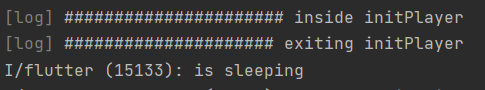
\includegraphics[width=\textwidth]{receive_kotlin_side.png}
			\caption{Sending data to Kotlin side Kotlin side}
		\end{subfigure}
		\hfill
		\begin{subfigure}[hbt!]{0.4\textwidth}
		         \centering
		         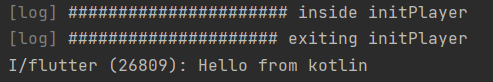
\includegraphics[width=\textwidth]{send_from_kotlin.png}
		         \caption{Receiving message from Kotlin side}
		     \end{subfigure}
		        \caption{Output}
		\end{figure}
		\end{enumerate}
	\item Install Google Fit on your phone. Record three activity sessions of your choice and fill in anthropometric data like weight, height or age. What other variables could be recorded?

	\begin{itemize}
		\item Gender
		\item Body fat
		\item Vitals (e.g. Blood pressure, Respiratory rate, etc.)
		\item etc.
	\end{itemize}
	\item Read through the different documentations of the Google Fit API. Explain what steps need to be taken to integrate the API to your project. The pipeline you design should help you to actually integrate the API in the next exercise session.

	From my point of view, the steps provided \href{https://developers.google.com/fit/android/get-started}{here} are sufficient. It doesn't make any sense to copy-paste it.
	\item Register your project

	From my point of view, the steps provided \href{https://developers.google.com/fit/android/get-api-key}{here} are sufficient. It doesn't make any sense to copy-paste it.
		\begin{figure}[hbt!]
			\centering
			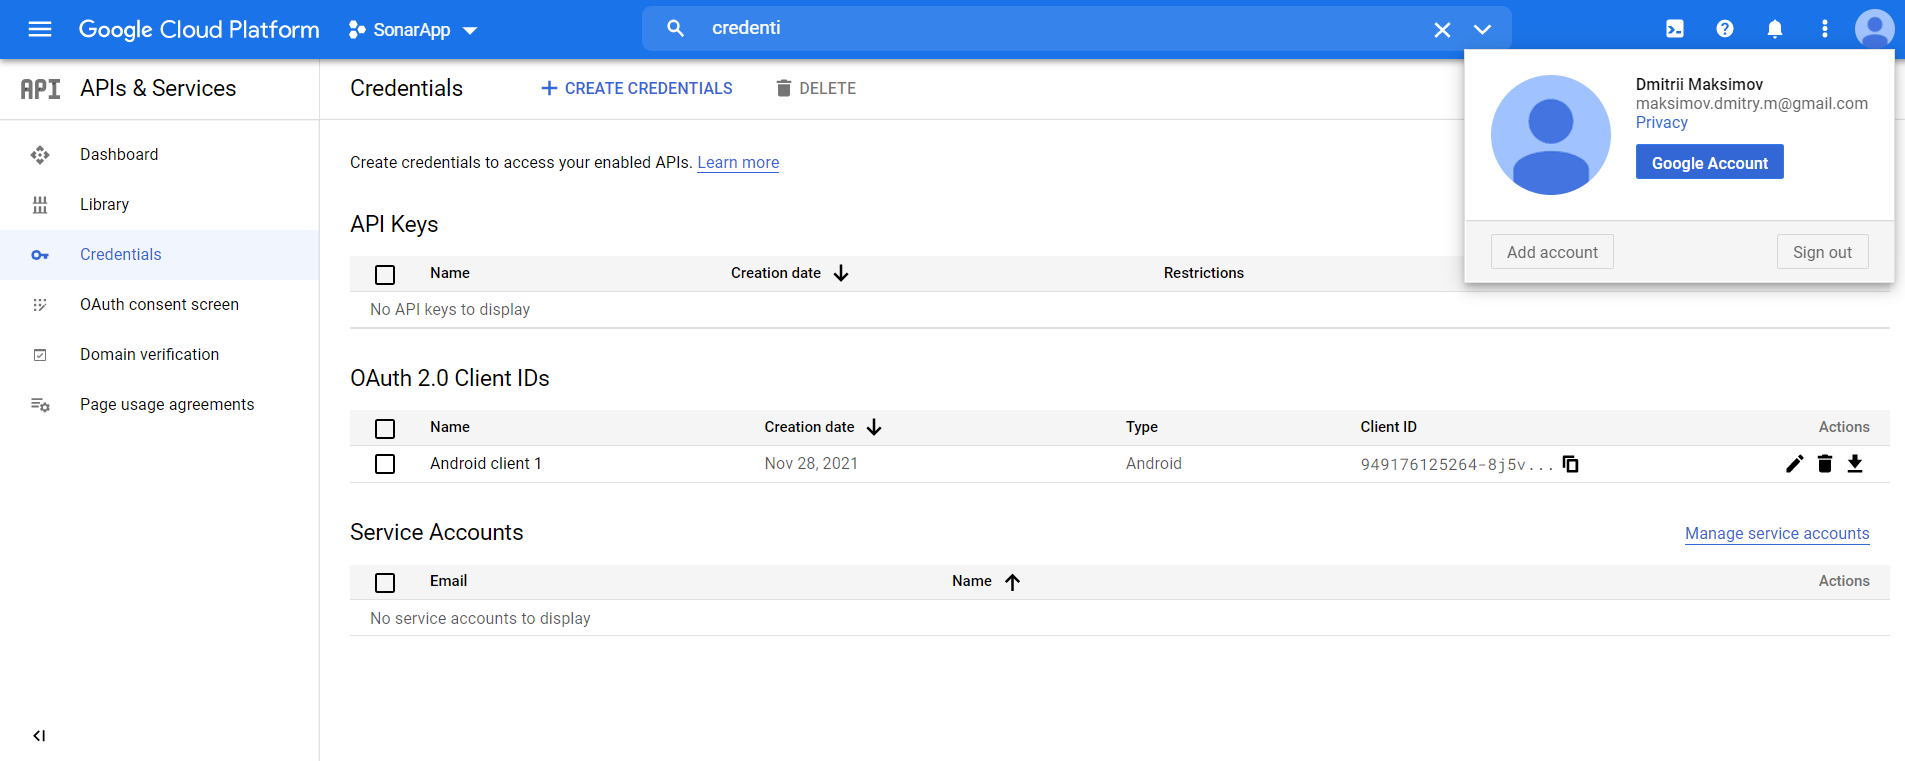
\includegraphics[width=1.\textwidth]{GReg.png}
			\caption{The proof of registration}
		\end{figure}

	\item Look at the documentation of the Fitness API. Which packages need to be imported and which other APIs might be needed for our purposes? Explain for each package why it would be needed.

	Packages:
	\begin{itemize}
		\item com.google.android.gms.fitness.Fitness. Since, it is the main entry point to Google Fit APIs.
		\item com.google.android.gms.fitness.FitnessActivities. This package are likely to be usefull. This is because recently we have recorded three activities.
		\item com.google.android.gms.fitness.FitnessOptions. To request permissions.
	\end{itemize}
	Other APIs:
	\begin{itemize}
		\item Sensors API. We can use different devices rather than only phone.
		\item Recording data. The sonar app should request automated storage of sensor data in a battery-efficient manner.
	\end{itemize}
	\item Develop a concept of how to migrate the data coming from the Sonar app to Google Fit. How need the data types to be converted? Are there some adjustments that have to be made in our app? If needed, feel free to make changes in the Sonar app. Explain why you make changes and document them. Use the following page as a starting point:
\end{enumerate}
\exercise
\begin{enumerate}
\item Rewrite your function which sends data from Flutter to Kotlin such that you can send results from the Sonar measurements. Explain how you convert the data. Is there a better way to convert the data?

The values types sended by invokeMethod are documented with StandardMessageCodec. Supported messages are acyclic values of these forms:
\begin{itemize}
	\item null
	\item bool
	\item num
	\item String
	\item List
	\item Map
\end{itemize}
In the tutorial we converted datetime data to string because StandardMessageCodec doesn't support this type.
\item Connect Google Fit and the Sonar App. Provide screenshots of your Google signin screen in the Sonar App and check if the Sonar App is found by Google Fit as a connected app. Also provide a screenshot of the connected apps in Google Fit including the Sonar app.

Unfortunately, I have faced the issue and can't deal with it:
\begin{figure}[hbt!]
	\centering
	\includegraphics[width=1.\textwidth]{ussue.png}
	\caption{Error}
\end{figure}
\item For our pipeline, data only needed to be written to Google Fit. Reading data was not needed. Explain conceptually how it is possible to read data using the History API.

In order to read data from Gogle Fit we have to use DataReadRequest class. This request should specify the time interval for the data and at least one data source or data type.
\item Choose an appropriate data type which can be used to send the Sonar data to Google Fit. Which data type do you choose? Does it need to be a sleep data type? Could also motion be tracked by our pipeline? Which usecase is more appropriate for the Sonar app?

Since we have bool variable sleep or not sleep, we can send sleep data type with a value of 2 if a person is sleeping and 1 otherwise. Using our pipeline, we can only determine whether it is sleep or not. Indeed, this is a more appropriate usecase for the Sonar app.
\item Provide screenshots of your Sonar App. Play a bit with the layout. Just change the background color and font types. Provide the code snippet which indicates where this needs to be changed as well as a screenshot of your layout.

\begin{figure}[hbt!]
	\centering
	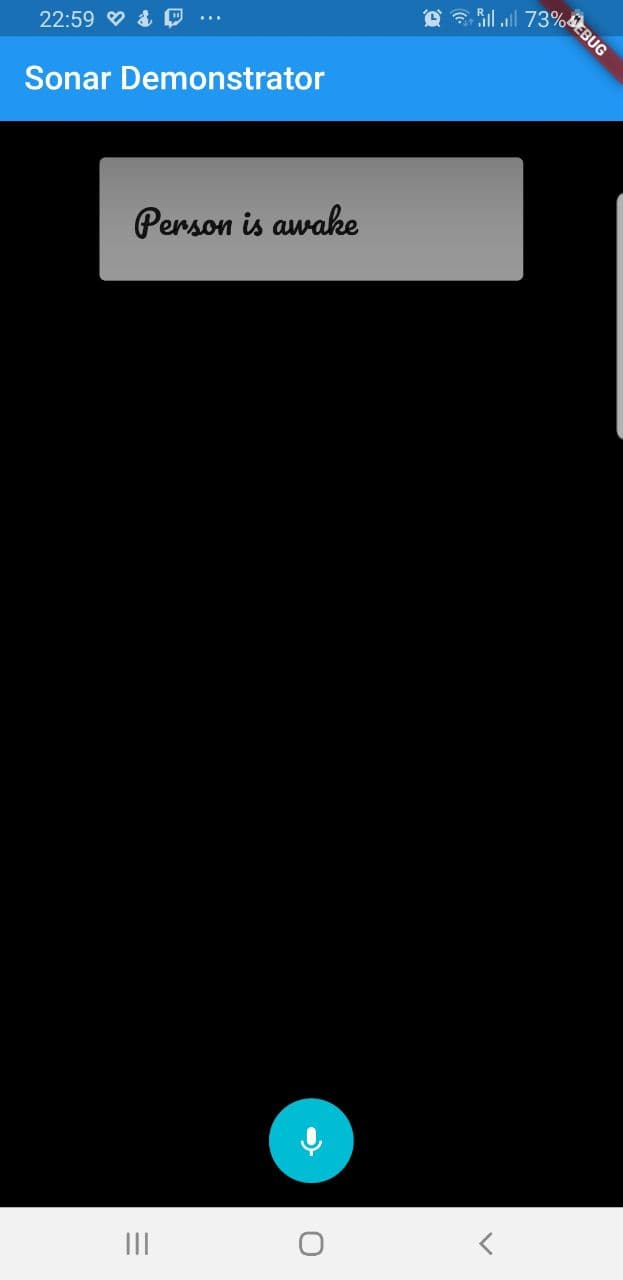
\includegraphics[width=0.5\textwidth]{screenshotjpg.jpg}
	\caption{Screenshot}
\end{figure}
	\begin{lstlisting}[language=Java, caption=Color and background settings in .dart file]
backgroundColor: Colors.black,
floatingActionButtonLocation: FloatingActionButtonLocation.centerFloat,
body:  Column(children: <Widget>[
AlertDialog(title: (sleeps) ? Text("Person is sleeping"):Text("Person is awake", style: GoogleFonts.pacifico()),backgroundColor:Colors.white60),
	\end{lstlisting}
\end{enumerate}

\end{document}